The MNIST dataset contains a total of $70000$ images of handwritten digits labeled with a number from $0$ to $9$. A predifined division of the dataset distinguishes $60000$ training examples and $10000$ test examples. Each image contains $28 \times 28 = 784$ pixels, where each pixel encodes the brightness in $8$ bit. The brightness of each pixel can be described by a variable $x_i \in \{0, 1, \dots, 255\}$ for $i \in \{1, 2, \dots, 784\}$. Hence, each image is completely defined by a vector of \textit{features}
\begin{align*}
\vec{x} = 
\begin{pmatrix}
x_1\\
x_2\\
\vdots\\
x_{784}
\end{pmatrix}.
\end{align*}
Each image $\vec{x}$ in the dataset is labeled with $y \in \{0, 1, \dots, 9\}$ that represents the handwritten digit displayed in the figure. The labels were decided by humans. In the present work, they are regarded as the \textit{true labels} in contrast to labels $\hat{y}$ predicted by an algorithm. So, every example in the dataset has the form $(\vec{x}, y)$.\\

In Figure~\ref{fig:plot_examples}, an examplary ensemble of ten different handwritten digits from $0$ to $9$ in the dataset is shown. 
\begin{figure}[h!]

\includegraphics[width=\textwidth]{plot_examples.pdf}
\caption{Examplary ensemble of ten different handwritten digits from $0$ to $9$ in the MNIST dataset. Each image can be described by a feature vector $\vec{x}$, and has a human-decided label $y$. The images consist of $28 \times 28 = 784$ pixels, where each pixel encodes an integer brightness level between $0$ and $255$.}
\label{fig:plot_examples}
\end{figure}

The decompistion of the $70000$ examples into training and test examples can be described by two sets $S$ (\textit{training set}) and $D$ (\textit{test set}). The training set $S$ contains all training examples $(\vec{x}, y)$, while the test set contains all test sets. There is no intersection between the sets $S$ and $D$, such that the test set contains images that are different from those in the training set. This allows the evaluation of the performance of a classification algorithm that was trained on the training set $S$.\\

Figure~\ref{fig:plot_hist_train} and Figure~\ref{fig:plot_hist_test} show a histogram of the frequency, with which each digit occurs in the training and test examples. Both the training and test set are balanced because the different digits appear with a similar frequency. In the following, this is important for the training of classifiers as there is no bias for a certain digit. 
\begin{figure}[h!]
    \begin{subfigure}[t]{0.5\textwidth}
        \centering
        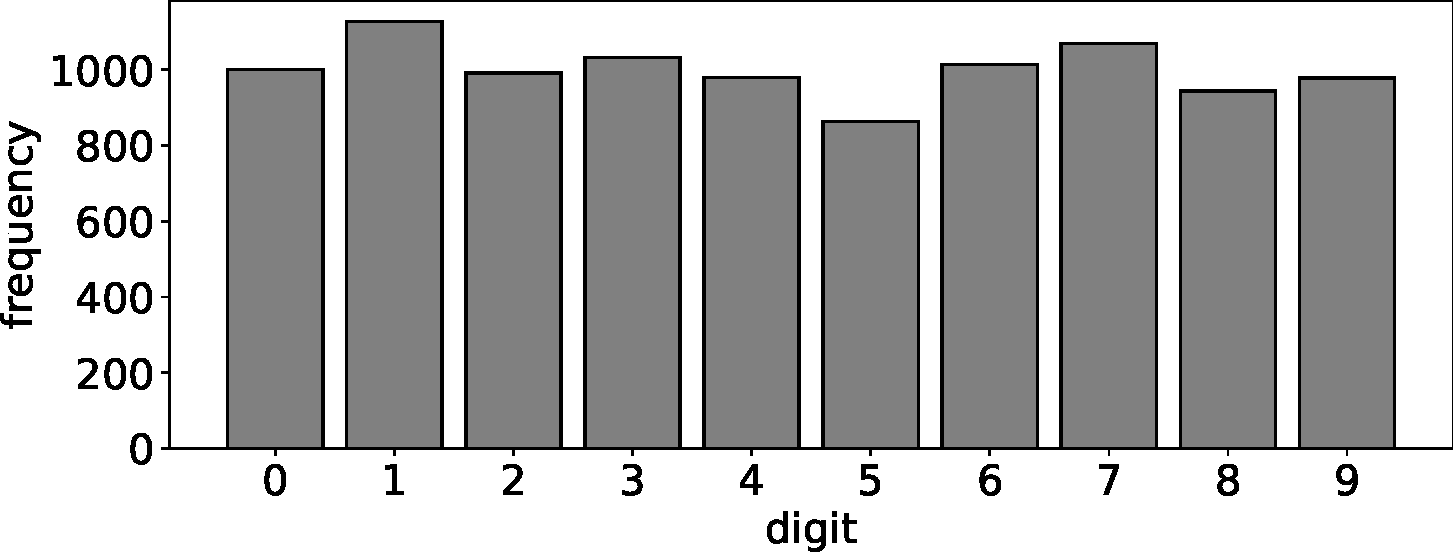
\includegraphics[width=\linewidth]{plot_hist_train.pdf} 
        \caption{training examples} \label{fig:plot_hist_train}
    \end{subfigure}
    \hfill
    \begin{subfigure}[t]{0.5\textwidth}
        \centering
        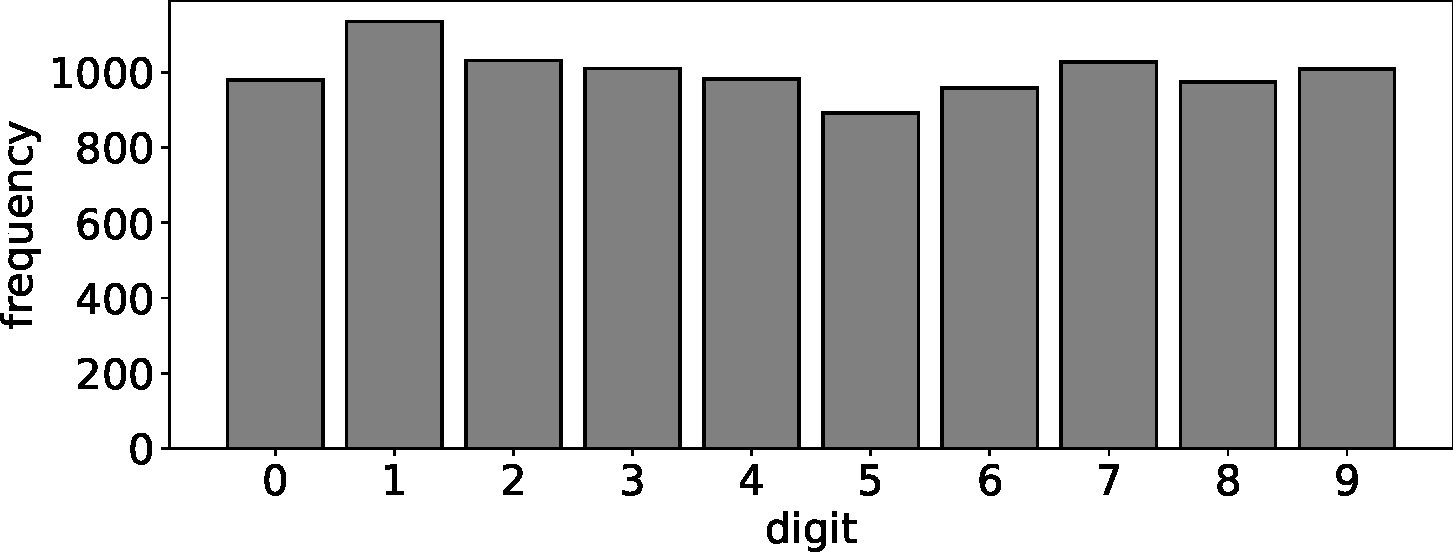
\includegraphics[width=\linewidth]{plot_hist_test.pdf} 
        \caption{test examples} \label{fig:plot_hist_test}
    \end{subfigure}
    \caption{The histogram shows, how often each digit occurs in (a) the training set $S$ and (b) the test set $D$. In both sets, all of the digits appear with a similar frequency, such that the training and test sets are balanced.}
\end{figure}


